% Created by tikzDevice version 0.7.0 on 2014-07-24 03:37:48
% !TEX encoding = UTF-8 Unicode
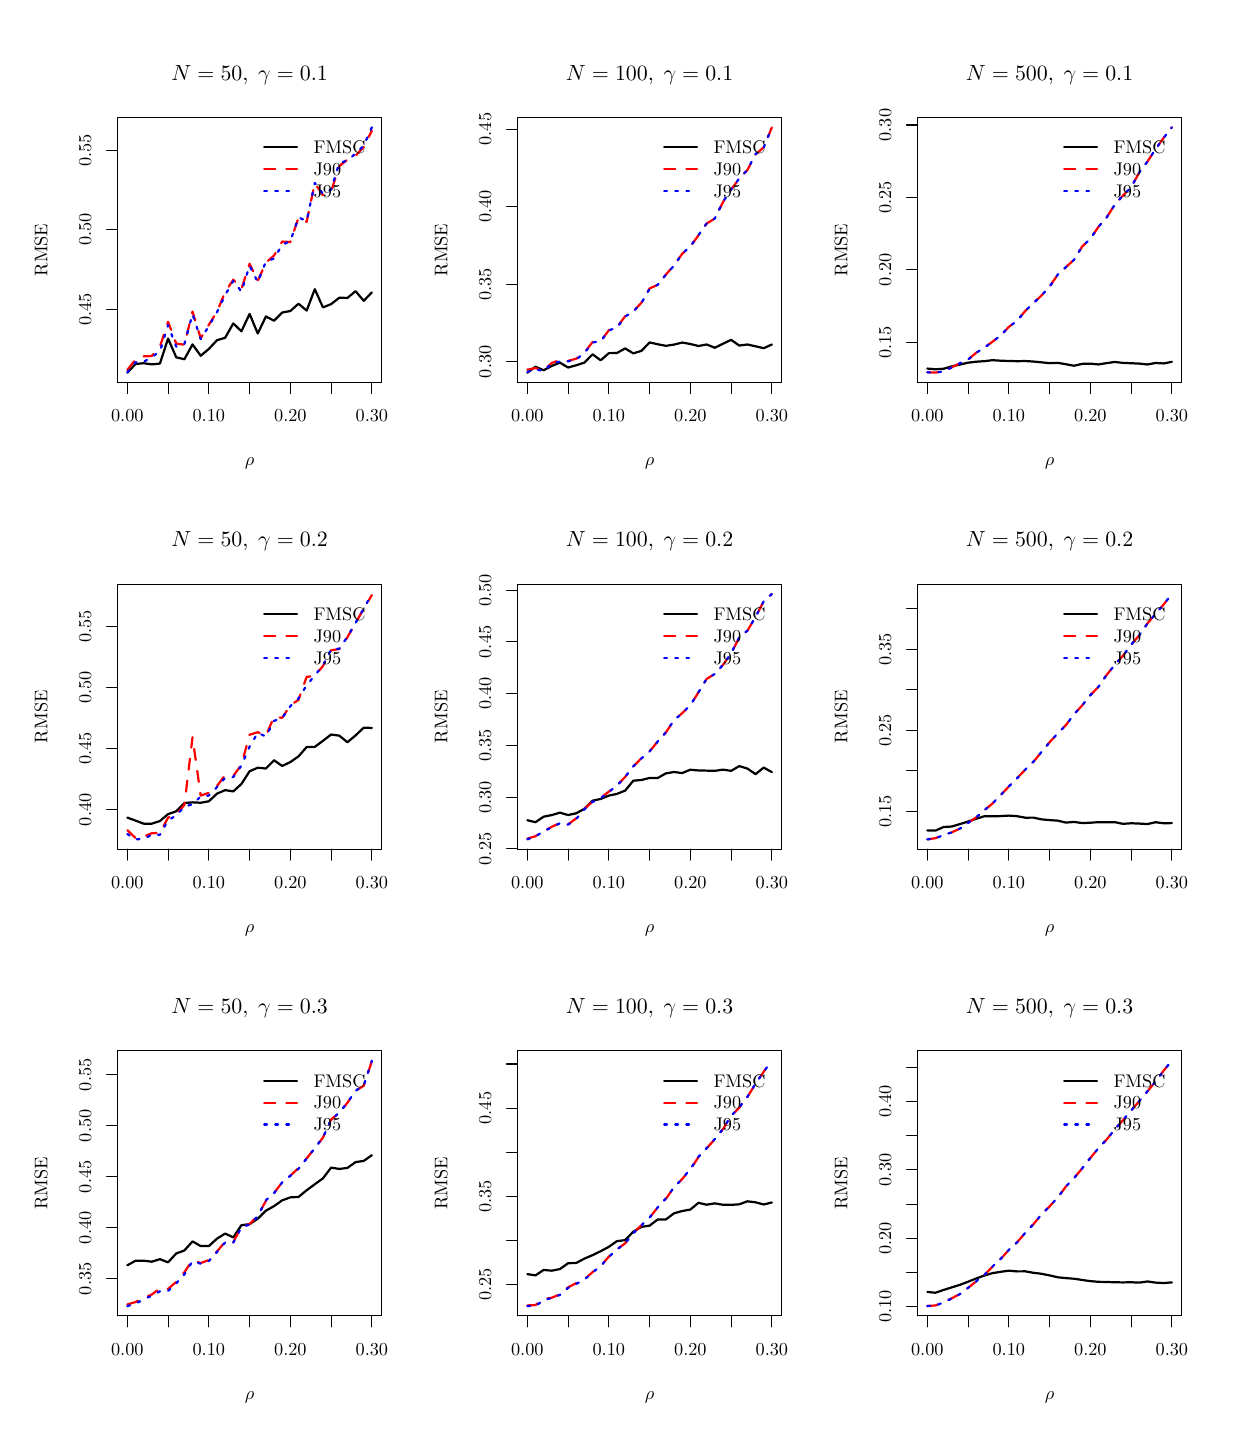
\begin{tikzpicture}[x=1pt,y=1pt]
\definecolor[named]{fillColor}{rgb}{1.00,1.00,1.00}
\path[use as bounding box,fill=fillColor,fill opacity=0.00] (0,0) rectangle (433.62,505.89);
\begin{scope}
\path[clip] ( 32.47,377.65) rectangle (127.91,473.42);
\definecolor[named]{drawColor}{rgb}{0.00,0.00,0.00}

\path[draw=drawColor,line width= 0.8pt,line join=round,line cap=round] ( 36.01,381.20) --
	( 38.95,384.35) --
	( 41.90,384.64) --
	( 44.84,384.21) --
	( 47.79,384.51) --
	( 50.73,393.53) --
	( 53.68,386.77) --
	( 56.63,386.08) --
	( 59.57,391.43) --
	( 62.52,387.34) --
	( 65.46,389.79) --
	( 68.41,392.95) --
	( 71.35,393.83) --
	( 74.30,399.02) --
	( 77.24,396.16) --
	( 80.19,402.46) --
	( 83.14,395.37) --
	( 86.08,401.52) --
	( 89.03,400.00) --
	( 91.97,402.95) --
	( 94.92,403.50) --
	( 97.86,406.14) --
	(100.81,403.67) --
	(103.75,411.39) --
	(106.70,404.80) --
	(109.65,405.99) --
	(112.59,408.30) --
	(115.54,408.23) --
	(118.48,410.67) --
	(121.43,407.19) --
	(124.37,410.23);
\end{scope}
\begin{scope}
\path[clip] (  0.00,  0.00) rectangle (433.62,505.89);
\definecolor[named]{drawColor}{rgb}{0.00,0.00,0.00}

\path[draw=drawColor,line width= 0.4pt,line join=round,line cap=round] ( 36.01,377.65) -- (124.37,377.65);

\path[draw=drawColor,line width= 0.4pt,line join=round,line cap=round] ( 36.01,377.65) -- ( 36.01,373.69);

\path[draw=drawColor,line width= 0.4pt,line join=round,line cap=round] ( 50.73,377.65) -- ( 50.73,373.69);

\path[draw=drawColor,line width= 0.4pt,line join=round,line cap=round] ( 65.46,377.65) -- ( 65.46,373.69);

\path[draw=drawColor,line width= 0.4pt,line join=round,line cap=round] ( 80.19,377.65) -- ( 80.19,373.69);

\path[draw=drawColor,line width= 0.4pt,line join=round,line cap=round] ( 94.92,377.65) -- ( 94.92,373.69);

\path[draw=drawColor,line width= 0.4pt,line join=round,line cap=round] (109.65,377.65) -- (109.65,373.69);

\path[draw=drawColor,line width= 0.4pt,line join=round,line cap=round] (124.37,377.65) -- (124.37,373.69);

\node[text=drawColor,anchor=base,inner sep=0pt, outer sep=0pt, scale=  0.66] at ( 36.01,363.40) {0.00};

\node[text=drawColor,anchor=base,inner sep=0pt, outer sep=0pt, scale=  0.66] at ( 65.46,363.40) {0.10};

\node[text=drawColor,anchor=base,inner sep=0pt, outer sep=0pt, scale=  0.66] at ( 94.92,363.40) {0.20};

\node[text=drawColor,anchor=base,inner sep=0pt, outer sep=0pt, scale=  0.66] at (124.37,363.40) {0.30};

\path[draw=drawColor,line width= 0.4pt,line join=round,line cap=round] ( 32.47,404.17) -- ( 32.47,461.56);

\path[draw=drawColor,line width= 0.4pt,line join=round,line cap=round] ( 32.47,404.17) -- ( 28.51,404.17);

\path[draw=drawColor,line width= 0.4pt,line join=round,line cap=round] ( 32.47,432.87) -- ( 28.51,432.87);

\path[draw=drawColor,line width= 0.4pt,line join=round,line cap=round] ( 32.47,461.56) -- ( 28.51,461.56);

\node[text=drawColor,rotate= 90.00,anchor=base,inner sep=0pt, outer sep=0pt, scale=  0.66] at ( 22.97,404.17) {0.45};

\node[text=drawColor,rotate= 90.00,anchor=base,inner sep=0pt, outer sep=0pt, scale=  0.66] at ( 22.97,432.87) {0.50};

\node[text=drawColor,rotate= 90.00,anchor=base,inner sep=0pt, outer sep=0pt, scale=  0.66] at ( 22.97,461.56) {0.55};

\path[draw=drawColor,line width= 0.4pt,line join=round,line cap=round] ( 32.47,377.65) --
	(127.91,377.65) --
	(127.91,473.42) --
	( 32.47,473.42) --
	( 32.47,377.65);
\end{scope}
\begin{scope}
\path[clip] (  0.00,337.26) rectangle (144.54,505.89);
\definecolor[named]{drawColor}{rgb}{0.00,0.00,0.00}

\node[text=drawColor,anchor=base,inner sep=0pt, outer sep=0pt, scale=  0.79] at ( 80.19,486.92) {\bfseries $N=50, \;\gamma=0.1$};

\node[text=drawColor,anchor=base,inner sep=0pt, outer sep=0pt, scale=  0.66] at ( 80.19,347.56) {$\rho$};

\node[text=drawColor,rotate= 90.00,anchor=base,inner sep=0pt, outer sep=0pt, scale=  0.66] at (  7.13,425.53) {RMSE};
\end{scope}
\begin{scope}
\path[clip] ( 32.47,377.65) rectangle (127.91,473.42);
\definecolor[named]{drawColor}{rgb}{1.00,0.00,0.00}

\path[draw=drawColor,line width= 0.8pt,dash pattern=on 4pt off 4pt ,line join=round,line cap=round] ( 36.01,382.17) --
	( 38.95,386.02) --
	( 41.90,387.12) --
	( 44.84,387.22) --
	( 47.79,390.59) --
	( 50.73,399.61) --
	( 53.68,391.70) --
	( 56.63,391.33) --
	( 59.57,403.31) --
	( 62.52,393.68) --
	( 65.46,398.50) --
	( 68.41,403.23) --
	( 71.35,410.34) --
	( 74.30,414.83) --
	( 77.24,411.51) --
	( 80.19,420.58) --
	( 83.14,414.42) --
	( 86.08,420.95) --
	( 89.03,423.56) --
	( 91.97,428.60) --
	( 94.92,428.42) --
	( 97.86,437.22) --
	(100.81,435.73) --
	(103.75,449.68) --
	(106.70,445.34) --
	(109.65,446.74) --
	(112.59,455.85) --
	(115.54,458.21) --
	(118.48,459.62) --
	(121.43,462.77) --
	(124.37,468.70);
\definecolor[named]{drawColor}{rgb}{0.00,0.00,1.00}

\path[draw=drawColor,line width= 0.8pt,dash pattern=on 1pt off 3pt ,line join=round,line cap=round] ( 36.01,381.35) --
	( 38.95,384.96) --
	( 41.90,385.11) --
	( 44.84,386.86) --
	( 47.79,388.88) --
	( 50.73,398.40) --
	( 53.68,390.62) --
	( 56.63,391.56) --
	( 59.57,402.39) --
	( 62.52,393.35) --
	( 65.46,398.08) --
	( 68.41,403.11) --
	( 71.35,409.27) --
	( 74.30,414.37) --
	( 77.24,410.54) --
	( 80.19,419.84) --
	( 83.14,413.92) --
	( 86.08,421.39) --
	( 89.03,422.48) --
	( 91.97,427.42) --
	( 94.92,428.78) --
	( 97.86,437.32) --
	(100.81,436.06) --
	(103.75,449.78) --
	(106.70,445.86) --
	(109.65,447.42) --
	(112.59,456.94) --
	(115.54,457.86) --
	(118.48,460.41) --
	(121.43,463.29) --
	(124.37,469.87);
\definecolor[named]{drawColor}{rgb}{0.00,0.00,0.00}

\path[draw=drawColor,line width= 0.8pt,line join=round,line cap=round] ( 85.47,462.63) -- ( 97.35,462.63);
\definecolor[named]{drawColor}{rgb}{1.00,0.00,0.00}

\path[draw=drawColor,line width= 0.8pt,dash pattern=on 4pt off 4pt ,line join=round,line cap=round] ( 85.47,454.71) -- ( 97.35,454.71);
\definecolor[named]{drawColor}{rgb}{0.00,0.00,1.00}

\path[draw=drawColor,line width= 0.8pt,dash pattern=on 1pt off 3pt ,line join=round,line cap=round] ( 85.47,446.79) -- ( 97.35,446.79);
\definecolor[named]{drawColor}{rgb}{0.00,0.00,0.00}

\node[text=drawColor,anchor=base west,inner sep=0pt, outer sep=0pt, scale=  0.66] at (103.29,460.35) {FMSC};

\node[text=drawColor,anchor=base west,inner sep=0pt, outer sep=0pt, scale=  0.66] at (103.29,452.43) {J90};

\node[text=drawColor,anchor=base west,inner sep=0pt, outer sep=0pt, scale=  0.66] at (103.29,444.51) {J95};
\end{scope}
\begin{scope}
\path[clip] (177.01,377.65) rectangle (272.45,473.42);
\definecolor[named]{drawColor}{rgb}{0.00,0.00,0.00}

\path[draw=drawColor,line width= 0.8pt,line join=round,line cap=round] (180.55,381.20) --
	(183.49,383.38) --
	(186.44,382.10) --
	(189.38,383.65) --
	(192.33,384.84) --
	(195.27,383.09) --
	(198.22,383.89) --
	(201.17,384.85) --
	(204.11,387.86) --
	(207.06,385.69) --
	(210.00,388.27) --
	(212.95,388.33) --
	(215.89,389.98) --
	(218.84,388.19) --
	(221.78,389.10) --
	(224.73,392.15) --
	(227.68,391.48) --
	(230.62,390.92) --
	(233.57,391.37) --
	(236.51,392.11) --
	(239.46,391.57) --
	(242.40,390.86) --
	(245.35,391.41) --
	(248.29,390.22) --
	(251.24,391.68) --
	(254.19,393.08) --
	(257.13,391.02) --
	(260.08,391.40) --
	(263.02,390.75) --
	(265.97,390.06) --
	(268.91,391.40);
\end{scope}
\begin{scope}
\path[clip] (  0.00,  0.00) rectangle (433.62,505.89);
\definecolor[named]{drawColor}{rgb}{0.00,0.00,0.00}

\path[draw=drawColor,line width= 0.4pt,line join=round,line cap=round] (180.55,377.65) -- (268.91,377.65);

\path[draw=drawColor,line width= 0.4pt,line join=round,line cap=round] (180.55,377.65) -- (180.55,373.69);

\path[draw=drawColor,line width= 0.4pt,line join=round,line cap=round] (195.27,377.65) -- (195.27,373.69);

\path[draw=drawColor,line width= 0.4pt,line join=round,line cap=round] (210.00,377.65) -- (210.00,373.69);

\path[draw=drawColor,line width= 0.4pt,line join=round,line cap=round] (224.73,377.65) -- (224.73,373.69);

\path[draw=drawColor,line width= 0.4pt,line join=round,line cap=round] (239.46,377.65) -- (239.46,373.69);

\path[draw=drawColor,line width= 0.4pt,line join=round,line cap=round] (254.19,377.65) -- (254.19,373.69);

\path[draw=drawColor,line width= 0.4pt,line join=round,line cap=round] (268.91,377.65) -- (268.91,373.69);

\node[text=drawColor,anchor=base,inner sep=0pt, outer sep=0pt, scale=  0.66] at (180.55,363.40) {0.00};

\node[text=drawColor,anchor=base,inner sep=0pt, outer sep=0pt, scale=  0.66] at (210.00,363.40) {0.10};

\node[text=drawColor,anchor=base,inner sep=0pt, outer sep=0pt, scale=  0.66] at (239.46,363.40) {0.20};

\node[text=drawColor,anchor=base,inner sep=0pt, outer sep=0pt, scale=  0.66] at (268.91,363.40) {0.30};

\path[draw=drawColor,line width= 0.4pt,line join=round,line cap=round] (177.01,385.13) -- (177.01,469.24);

\path[draw=drawColor,line width= 0.4pt,line join=round,line cap=round] (177.01,385.13) -- (173.05,385.13);

\path[draw=drawColor,line width= 0.4pt,line join=round,line cap=round] (177.01,413.17) -- (173.05,413.17);

\path[draw=drawColor,line width= 0.4pt,line join=round,line cap=round] (177.01,441.20) -- (173.05,441.20);

\path[draw=drawColor,line width= 0.4pt,line join=round,line cap=round] (177.01,469.24) -- (173.05,469.24);

\node[text=drawColor,rotate= 90.00,anchor=base,inner sep=0pt, outer sep=0pt, scale=  0.66] at (167.51,385.13) {0.30};

\node[text=drawColor,rotate= 90.00,anchor=base,inner sep=0pt, outer sep=0pt, scale=  0.66] at (167.51,413.17) {0.35};

\node[text=drawColor,rotate= 90.00,anchor=base,inner sep=0pt, outer sep=0pt, scale=  0.66] at (167.51,441.20) {0.40};

\node[text=drawColor,rotate= 90.00,anchor=base,inner sep=0pt, outer sep=0pt, scale=  0.66] at (167.51,469.24) {0.45};

\path[draw=drawColor,line width= 0.4pt,line join=round,line cap=round] (177.01,377.65) --
	(272.45,377.65) --
	(272.45,473.42) --
	(177.01,473.42) --
	(177.01,377.65);
\end{scope}
\begin{scope}
\path[clip] (144.54,337.26) rectangle (289.08,505.89);
\definecolor[named]{drawColor}{rgb}{0.00,0.00,0.00}

\node[text=drawColor,anchor=base,inner sep=0pt, outer sep=0pt, scale=  0.79] at (224.73,486.92) {\bfseries $N=100, \;\gamma=0.1$};

\node[text=drawColor,anchor=base,inner sep=0pt, outer sep=0pt, scale=  0.66] at (224.73,347.56) {$\rho$};

\node[text=drawColor,rotate= 90.00,anchor=base,inner sep=0pt, outer sep=0pt, scale=  0.66] at (151.67,425.53) {RMSE};
\end{scope}
\begin{scope}
\path[clip] (177.01,377.65) rectangle (272.45,473.42);
\definecolor[named]{drawColor}{rgb}{1.00,0.00,0.00}

\path[draw=drawColor,line width= 0.8pt,dash pattern=on 4pt off 4pt ,line join=round,line cap=round] (180.55,382.31) --
	(183.49,382.87) --
	(186.44,381.97) --
	(189.38,384.74) --
	(192.33,385.75) --
	(195.27,385.47) --
	(198.22,386.27) --
	(201.17,388.46) --
	(204.11,392.27) --
	(207.06,392.61) --
	(210.00,396.56) --
	(212.95,397.65) --
	(215.89,401.61) --
	(218.84,403.32) --
	(221.78,406.52) --
	(224.73,411.67) --
	(227.68,412.97) --
	(230.62,416.67) --
	(233.57,420.03) --
	(236.51,424.18) --
	(239.46,426.78) --
	(242.40,430.88) --
	(245.35,435.10) --
	(248.29,436.92) --
	(251.24,442.84) --
	(254.19,447.39) --
	(257.13,451.34) --
	(260.08,454.45) --
	(263.02,460.10) --
	(265.97,462.66) --
	(268.91,469.83);
\definecolor[named]{drawColor}{rgb}{0.00,0.00,1.00}

\path[draw=drawColor,line width= 0.8pt,dash pattern=on 1pt off 3pt ,line join=round,line cap=round] (180.55,381.50) --
	(183.49,382.47) --
	(186.44,381.77) --
	(189.38,384.57) --
	(192.33,385.23) --
	(195.27,385.31) --
	(198.22,386.05) --
	(201.17,388.31) --
	(204.11,392.13) --
	(207.06,392.58) --
	(210.00,396.49) --
	(212.95,397.52) --
	(215.89,401.50) --
	(218.84,403.33) --
	(221.78,406.43) --
	(224.73,411.47) --
	(227.68,413.00) --
	(230.62,416.60) --
	(233.57,419.92) --
	(236.51,424.19) --
	(239.46,426.87) --
	(242.40,430.90) --
	(245.35,435.17) --
	(248.29,436.94) --
	(251.24,442.91) --
	(254.19,447.44) --
	(257.13,451.41) --
	(260.08,454.52) --
	(263.02,460.20) --
	(265.97,462.57) --
	(268.91,469.87);
\definecolor[named]{drawColor}{rgb}{0.00,0.00,0.00}

\path[draw=drawColor,line width= 0.8pt,line join=round,line cap=round] (230.01,462.63) -- (241.89,462.63);
\definecolor[named]{drawColor}{rgb}{1.00,0.00,0.00}

\path[draw=drawColor,line width= 0.8pt,dash pattern=on 4pt off 4pt ,line join=round,line cap=round] (230.01,454.71) -- (241.89,454.71);
\definecolor[named]{drawColor}{rgb}{0.00,0.00,1.00}

\path[draw=drawColor,line width= 0.8pt,dash pattern=on 1pt off 3pt ,line join=round,line cap=round] (230.01,446.79) -- (241.89,446.79);
\definecolor[named]{drawColor}{rgb}{0.00,0.00,0.00}

\node[text=drawColor,anchor=base west,inner sep=0pt, outer sep=0pt, scale=  0.66] at (247.83,460.35) {FMSC};

\node[text=drawColor,anchor=base west,inner sep=0pt, outer sep=0pt, scale=  0.66] at (247.83,452.43) {J90};

\node[text=drawColor,anchor=base west,inner sep=0pt, outer sep=0pt, scale=  0.66] at (247.83,444.51) {J95};
\end{scope}
\begin{scope}
\path[clip] (321.55,377.65) rectangle (416.99,473.42);
\definecolor[named]{drawColor}{rgb}{0.00,0.00,0.00}

\path[draw=drawColor,line width= 0.8pt,line join=round,line cap=round] (325.09,382.70) --
	(328.03,382.45) --
	(330.98,382.64) --
	(333.92,383.51) --
	(336.87,384.14) --
	(339.81,384.83) --
	(342.76,385.18) --
	(345.71,385.38) --
	(348.65,385.73) --
	(351.60,385.54) --
	(354.54,385.45) --
	(357.49,385.37) --
	(360.43,385.42) --
	(363.38,385.25) --
	(366.32,384.95) --
	(369.27,384.66) --
	(372.22,384.77) --
	(375.16,384.27) --
	(378.11,383.72) --
	(381.05,384.40) --
	(384.00,384.49) --
	(386.94,384.19) --
	(389.89,384.68) --
	(392.83,385.09) --
	(395.78,384.75) --
	(398.73,384.63) --
	(401.67,384.50) --
	(404.62,384.18) --
	(407.56,384.72) --
	(410.51,384.56) --
	(413.45,385.14);
\end{scope}
\begin{scope}
\path[clip] (  0.00,  0.00) rectangle (433.62,505.89);
\definecolor[named]{drawColor}{rgb}{0.00,0.00,0.00}

\path[draw=drawColor,line width= 0.4pt,line join=round,line cap=round] (325.09,377.65) -- (413.45,377.65);

\path[draw=drawColor,line width= 0.4pt,line join=round,line cap=round] (325.09,377.65) -- (325.09,373.69);

\path[draw=drawColor,line width= 0.4pt,line join=round,line cap=round] (339.81,377.65) -- (339.81,373.69);

\path[draw=drawColor,line width= 0.4pt,line join=round,line cap=round] (354.54,377.65) -- (354.54,373.69);

\path[draw=drawColor,line width= 0.4pt,line join=round,line cap=round] (369.27,377.65) -- (369.27,373.69);

\path[draw=drawColor,line width= 0.4pt,line join=round,line cap=round] (384.00,377.65) -- (384.00,373.69);

\path[draw=drawColor,line width= 0.4pt,line join=round,line cap=round] (398.73,377.65) -- (398.73,373.69);

\path[draw=drawColor,line width= 0.4pt,line join=round,line cap=round] (413.45,377.65) -- (413.45,373.69);

\node[text=drawColor,anchor=base,inner sep=0pt, outer sep=0pt, scale=  0.66] at (325.09,363.40) {0.00};

\node[text=drawColor,anchor=base,inner sep=0pt, outer sep=0pt, scale=  0.66] at (354.54,363.40) {0.10};

\node[text=drawColor,anchor=base,inner sep=0pt, outer sep=0pt, scale=  0.66] at (384.00,363.40) {0.20};

\node[text=drawColor,anchor=base,inner sep=0pt, outer sep=0pt, scale=  0.66] at (413.45,363.40) {0.30};

\path[draw=drawColor,line width= 0.4pt,line join=round,line cap=round] (321.55,392.23) -- (321.55,470.71);

\path[draw=drawColor,line width= 0.4pt,line join=round,line cap=round] (321.55,392.23) -- (317.59,392.23);

\path[draw=drawColor,line width= 0.4pt,line join=round,line cap=round] (321.55,418.39) -- (317.59,418.39);

\path[draw=drawColor,line width= 0.4pt,line join=round,line cap=round] (321.55,444.55) -- (317.59,444.55);

\path[draw=drawColor,line width= 0.4pt,line join=round,line cap=round] (321.55,470.71) -- (317.59,470.71);

\node[text=drawColor,rotate= 90.00,anchor=base,inner sep=0pt, outer sep=0pt, scale=  0.66] at (312.05,392.23) {0.15};

\node[text=drawColor,rotate= 90.00,anchor=base,inner sep=0pt, outer sep=0pt, scale=  0.66] at (312.05,418.39) {0.20};

\node[text=drawColor,rotate= 90.00,anchor=base,inner sep=0pt, outer sep=0pt, scale=  0.66] at (312.05,444.55) {0.25};

\node[text=drawColor,rotate= 90.00,anchor=base,inner sep=0pt, outer sep=0pt, scale=  0.66] at (312.05,470.71) {0.30};

\path[draw=drawColor,line width= 0.4pt,line join=round,line cap=round] (321.55,377.65) --
	(416.99,377.65) --
	(416.99,473.42) --
	(321.55,473.42) --
	(321.55,377.65);
\end{scope}
\begin{scope}
\path[clip] (289.08,337.26) rectangle (433.62,505.89);
\definecolor[named]{drawColor}{rgb}{0.00,0.00,0.00}

\node[text=drawColor,anchor=base,inner sep=0pt, outer sep=0pt, scale=  0.79] at (369.27,486.92) {\bfseries $N=500, \;\gamma=0.1$};

\node[text=drawColor,anchor=base,inner sep=0pt, outer sep=0pt, scale=  0.66] at (369.27,347.56) {$\rho$};

\node[text=drawColor,rotate= 90.00,anchor=base,inner sep=0pt, outer sep=0pt, scale=  0.66] at (296.21,425.53) {RMSE};
\end{scope}
\begin{scope}
\path[clip] (321.55,377.65) rectangle (416.99,473.42);
\definecolor[named]{drawColor}{rgb}{1.00,0.00,0.00}

\path[draw=drawColor,line width= 0.8pt,dash pattern=on 4pt off 4pt ,line join=round,line cap=round] (325.09,381.38) --
	(328.03,381.23) --
	(330.98,381.76) --
	(333.92,383.14) --
	(336.87,384.67) --
	(339.81,385.93) --
	(342.76,388.45) --
	(345.71,390.25) --
	(348.65,392.44) --
	(351.60,394.63) --
	(354.54,397.77) --
	(357.49,399.90) --
	(360.43,403.50) --
	(363.38,406.28) --
	(366.32,409.10) --
	(369.27,412.32) --
	(372.22,416.67) --
	(375.16,419.33) --
	(378.11,422.06) --
	(381.05,426.82) --
	(384.00,429.62) --
	(386.94,433.95) --
	(389.89,437.32) --
	(392.83,441.96) --
	(395.78,445.24) --
	(398.73,448.25) --
	(401.67,453.52) --
	(404.62,457.48) --
	(407.56,461.99) --
	(410.51,466.12) --
	(413.45,469.87);
\definecolor[named]{drawColor}{rgb}{0.00,0.00,1.00}

\path[draw=drawColor,line width= 0.8pt,dash pattern=on 1pt off 3pt ,line join=round,line cap=round] (325.09,381.36) --
	(328.03,381.20) --
	(330.98,381.74) --
	(333.92,383.12) --
	(336.87,384.66) --
	(339.81,385.96) --
	(342.76,388.44) --
	(345.71,390.24) --
	(348.65,392.45) --
	(351.60,394.63) --
	(354.54,397.78) --
	(357.49,399.91) --
	(360.43,403.50) --
	(363.38,406.28) --
	(366.32,409.10) --
	(369.27,412.32) --
	(372.22,416.67) --
	(375.16,419.33) --
	(378.11,422.06) --
	(381.05,426.82) --
	(384.00,429.62) --
	(386.94,433.95) --
	(389.89,437.32) --
	(392.83,441.96) --
	(395.78,445.24) --
	(398.73,448.25) --
	(401.67,453.52) --
	(404.62,457.48) --
	(407.56,461.99) --
	(410.51,466.12) --
	(413.45,469.87);
\definecolor[named]{drawColor}{rgb}{0.00,0.00,0.00}

\path[draw=drawColor,line width= 0.8pt,line join=round,line cap=round] (374.55,462.63) -- (386.43,462.63);
\definecolor[named]{drawColor}{rgb}{1.00,0.00,0.00}

\path[draw=drawColor,line width= 0.8pt,dash pattern=on 4pt off 4pt ,line join=round,line cap=round] (374.55,454.71) -- (386.43,454.71);
\definecolor[named]{drawColor}{rgb}{0.00,0.00,1.00}

\path[draw=drawColor,line width= 0.8pt,dash pattern=on 1pt off 3pt ,line join=round,line cap=round] (374.55,446.79) -- (386.43,446.79);
\definecolor[named]{drawColor}{rgb}{0.00,0.00,0.00}

\node[text=drawColor,anchor=base west,inner sep=0pt, outer sep=0pt, scale=  0.66] at (392.37,460.35) {FMSC};

\node[text=drawColor,anchor=base west,inner sep=0pt, outer sep=0pt, scale=  0.66] at (392.37,452.43) {J90};

\node[text=drawColor,anchor=base west,inner sep=0pt, outer sep=0pt, scale=  0.66] at (392.37,444.51) {J95};
\end{scope}
\begin{scope}
\path[clip] ( 32.47,209.02) rectangle (127.91,304.79);
\definecolor[named]{drawColor}{rgb}{0.00,0.00,0.00}

\path[draw=drawColor,line width= 0.8pt,line join=round,line cap=round] ( 36.01,220.45) --
	( 38.95,219.37) --
	( 41.90,218.26) --
	( 44.84,218.26) --
	( 47.79,219.20) --
	( 50.73,221.72) --
	( 53.68,222.71) --
	( 56.63,225.71) --
	( 59.57,225.96) --
	( 62.52,225.81) --
	( 65.46,226.34) --
	( 68.41,229.10) --
	( 71.35,230.37) --
	( 74.30,229.91) --
	( 77.24,232.61) --
	( 80.19,237.18) --
	( 83.14,238.48) --
	( 86.08,238.18) --
	( 89.03,241.17) --
	( 91.97,239.10) --
	( 94.92,240.52) --
	( 97.86,242.57) --
	(100.81,245.95) --
	(103.75,246.00) --
	(106.70,248.20) --
	(109.65,250.47) --
	(112.59,250.06) --
	(115.54,247.68) --
	(118.48,250.14) --
	(121.43,252.94) --
	(124.37,252.84);
\end{scope}
\begin{scope}
\path[clip] (  0.00,  0.00) rectangle (433.62,505.89);
\definecolor[named]{drawColor}{rgb}{0.00,0.00,0.00}

\path[draw=drawColor,line width= 0.4pt,line join=round,line cap=round] ( 36.01,209.02) -- (124.37,209.02);

\path[draw=drawColor,line width= 0.4pt,line join=round,line cap=round] ( 36.01,209.02) -- ( 36.01,205.06);

\path[draw=drawColor,line width= 0.4pt,line join=round,line cap=round] ( 50.73,209.02) -- ( 50.73,205.06);

\path[draw=drawColor,line width= 0.4pt,line join=round,line cap=round] ( 65.46,209.02) -- ( 65.46,205.06);

\path[draw=drawColor,line width= 0.4pt,line join=round,line cap=round] ( 80.19,209.02) -- ( 80.19,205.06);

\path[draw=drawColor,line width= 0.4pt,line join=round,line cap=round] ( 94.92,209.02) -- ( 94.92,205.06);

\path[draw=drawColor,line width= 0.4pt,line join=round,line cap=round] (109.65,209.02) -- (109.65,205.06);

\path[draw=drawColor,line width= 0.4pt,line join=round,line cap=round] (124.37,209.02) -- (124.37,205.06);

\node[text=drawColor,anchor=base,inner sep=0pt, outer sep=0pt, scale=  0.66] at ( 36.01,194.77) {0.00};

\node[text=drawColor,anchor=base,inner sep=0pt, outer sep=0pt, scale=  0.66] at ( 65.46,194.77) {0.10};

\node[text=drawColor,anchor=base,inner sep=0pt, outer sep=0pt, scale=  0.66] at ( 94.92,194.77) {0.20};

\node[text=drawColor,anchor=base,inner sep=0pt, outer sep=0pt, scale=  0.66] at (124.37,194.77) {0.30};

\path[draw=drawColor,line width= 0.4pt,line join=round,line cap=round] ( 32.47,223.26) -- ( 32.47,289.59);

\path[draw=drawColor,line width= 0.4pt,line join=round,line cap=round] ( 32.47,223.26) -- ( 28.51,223.26);

\path[draw=drawColor,line width= 0.4pt,line join=round,line cap=round] ( 32.47,245.37) -- ( 28.51,245.37);

\path[draw=drawColor,line width= 0.4pt,line join=round,line cap=round] ( 32.47,267.48) -- ( 28.51,267.48);

\path[draw=drawColor,line width= 0.4pt,line join=round,line cap=round] ( 32.47,289.59) -- ( 28.51,289.59);

\node[text=drawColor,rotate= 90.00,anchor=base,inner sep=0pt, outer sep=0pt, scale=  0.66] at ( 22.97,223.26) {0.40};

\node[text=drawColor,rotate= 90.00,anchor=base,inner sep=0pt, outer sep=0pt, scale=  0.66] at ( 22.97,245.37) {0.45};

\node[text=drawColor,rotate= 90.00,anchor=base,inner sep=0pt, outer sep=0pt, scale=  0.66] at ( 22.97,267.48) {0.50};

\node[text=drawColor,rotate= 90.00,anchor=base,inner sep=0pt, outer sep=0pt, scale=  0.66] at ( 22.97,289.59) {0.55};

\path[draw=drawColor,line width= 0.4pt,line join=round,line cap=round] ( 32.47,209.02) --
	(127.91,209.02) --
	(127.91,304.79) --
	( 32.47,304.79) --
	( 32.47,209.02);
\end{scope}
\begin{scope}
\path[clip] (  0.00,168.63) rectangle (144.54,337.26);
\definecolor[named]{drawColor}{rgb}{0.00,0.00,0.00}

\node[text=drawColor,anchor=base,inner sep=0pt, outer sep=0pt, scale=  0.79] at ( 80.19,318.29) {\bfseries $N=50, \;\gamma=0.2$};

\node[text=drawColor,anchor=base,inner sep=0pt, outer sep=0pt, scale=  0.66] at ( 80.19,178.93) {$\rho$};

\node[text=drawColor,rotate= 90.00,anchor=base,inner sep=0pt, outer sep=0pt, scale=  0.66] at (  7.13,256.90) {RMSE};
\end{scope}
\begin{scope}
\path[clip] ( 32.47,209.02) rectangle (127.91,304.79);
\definecolor[named]{drawColor}{rgb}{1.00,0.00,0.00}

\path[draw=drawColor,line width= 0.8pt,dash pattern=on 4pt off 4pt ,line join=round,line cap=round] ( 36.01,215.91) --
	( 38.95,213.09) --
	( 41.90,213.57) --
	( 44.84,214.79) --
	( 47.79,214.91) --
	( 50.73,220.44) --
	( 53.68,221.58) --
	( 56.63,225.04) --
	( 59.57,249.45) --
	( 62.52,228.40) --
	( 65.46,229.38) --
	( 68.41,231.82) --
	( 71.35,235.85) --
	( 74.30,235.48) --
	( 77.24,239.55) --
	( 80.19,250.38) --
	( 83.14,251.30) --
	( 86.08,250.01) --
	( 89.03,256.91) --
	( 91.97,256.49) --
	( 94.92,261.05) --
	( 97.86,262.99) --
	(100.81,271.30) --
	(103.75,271.67) --
	(106.70,275.21) --
	(109.65,280.93) --
	(112.59,281.34) --
	(115.54,285.59) --
	(118.48,290.79) --
	(121.43,295.84) --
	(124.37,300.86);
\definecolor[named]{drawColor}{rgb}{0.00,0.00,1.00}

\path[draw=drawColor,line width= 0.8pt,dash pattern=on 1pt off 3pt ,line join=round,line cap=round] ( 36.01,214.52) --
	( 38.95,212.57) --
	( 41.90,212.80) --
	( 44.84,214.22) --
	( 47.79,214.23) --
	( 50.73,219.49) --
	( 53.68,221.19) --
	( 56.63,224.41) --
	( 59.57,225.25) --
	( 62.52,228.05) --
	( 65.46,228.41) --
	( 68.41,231.48) --
	( 71.35,234.84) --
	( 74.30,235.10) --
	( 77.24,239.23) --
	( 80.19,246.11) --
	( 83.14,251.03) --
	( 86.08,249.79) --
	( 89.03,255.40) --
	( 91.97,256.44) --
	( 94.92,260.71) --
	( 97.86,263.53) --
	(100.81,268.26) --
	(103.75,271.81) --
	(106.70,275.50) --
	(109.65,281.24) --
	(112.59,281.50) --
	(115.54,285.79) --
	(118.48,290.80) --
	(121.43,295.99) --
	(124.37,301.24);
\definecolor[named]{drawColor}{rgb}{0.00,0.00,0.00}

\path[draw=drawColor,line width= 0.8pt,line join=round,line cap=round] ( 85.47,294.00) -- ( 97.35,294.00);
\definecolor[named]{drawColor}{rgb}{1.00,0.00,0.00}

\path[draw=drawColor,line width= 0.8pt,dash pattern=on 4pt off 4pt ,line join=round,line cap=round] ( 85.47,286.08) -- ( 97.35,286.08);
\definecolor[named]{drawColor}{rgb}{0.00,0.00,1.00}

\path[draw=drawColor,line width= 0.8pt,dash pattern=on 1pt off 3pt ,line join=round,line cap=round] ( 85.47,278.16) -- ( 97.35,278.16);
\definecolor[named]{drawColor}{rgb}{0.00,0.00,0.00}

\node[text=drawColor,anchor=base west,inner sep=0pt, outer sep=0pt, scale=  0.66] at (103.29,291.72) {FMSC};

\node[text=drawColor,anchor=base west,inner sep=0pt, outer sep=0pt, scale=  0.66] at (103.29,283.80) {J90};

\node[text=drawColor,anchor=base west,inner sep=0pt, outer sep=0pt, scale=  0.66] at (103.29,275.88) {J95};
\end{scope}
\begin{scope}
\path[clip] (177.01,209.02) rectangle (272.45,304.79);
\definecolor[named]{drawColor}{rgb}{0.00,0.00,0.00}

\path[draw=drawColor,line width= 0.8pt,line join=round,line cap=round] (180.55,219.50) --
	(183.49,218.78) --
	(186.44,220.78) --
	(189.38,221.36) --
	(192.33,222.24) --
	(195.27,221.37) --
	(198.22,222.01) --
	(201.17,223.63) --
	(204.11,226.55) --
	(207.06,227.19) --
	(210.00,228.39) --
	(212.95,229.03) --
	(215.89,230.19) --
	(218.84,233.78) --
	(221.78,234.04) --
	(224.73,234.77) --
	(227.68,234.78) --
	(230.62,236.43) --
	(233.57,236.92) --
	(236.51,236.54) --
	(239.46,237.75) --
	(242.40,237.48) --
	(245.35,237.42) --
	(248.29,237.34) --
	(251.24,237.78) --
	(254.19,237.34) --
	(257.13,239.05) --
	(260.08,238.16) --
	(263.02,236.15) --
	(265.97,238.53) --
	(268.91,236.88);
\end{scope}
\begin{scope}
\path[clip] (  0.00,  0.00) rectangle (433.62,505.89);
\definecolor[named]{drawColor}{rgb}{0.00,0.00,0.00}

\path[draw=drawColor,line width= 0.4pt,line join=round,line cap=round] (180.55,209.02) -- (268.91,209.02);

\path[draw=drawColor,line width= 0.4pt,line join=round,line cap=round] (180.55,209.02) -- (180.55,205.06);

\path[draw=drawColor,line width= 0.4pt,line join=round,line cap=round] (195.27,209.02) -- (195.27,205.06);

\path[draw=drawColor,line width= 0.4pt,line join=round,line cap=round] (210.00,209.02) -- (210.00,205.06);

\path[draw=drawColor,line width= 0.4pt,line join=round,line cap=round] (224.73,209.02) -- (224.73,205.06);

\path[draw=drawColor,line width= 0.4pt,line join=round,line cap=round] (239.46,209.02) -- (239.46,205.06);

\path[draw=drawColor,line width= 0.4pt,line join=round,line cap=round] (254.19,209.02) -- (254.19,205.06);

\path[draw=drawColor,line width= 0.4pt,line join=round,line cap=round] (268.91,209.02) -- (268.91,205.06);

\node[text=drawColor,anchor=base,inner sep=0pt, outer sep=0pt, scale=  0.66] at (180.55,194.77) {0.00};

\node[text=drawColor,anchor=base,inner sep=0pt, outer sep=0pt, scale=  0.66] at (210.00,194.77) {0.10};

\node[text=drawColor,anchor=base,inner sep=0pt, outer sep=0pt, scale=  0.66] at (239.46,194.77) {0.20};

\node[text=drawColor,anchor=base,inner sep=0pt, outer sep=0pt, scale=  0.66] at (268.91,194.77) {0.30};

\path[draw=drawColor,line width= 0.4pt,line join=round,line cap=round] (177.01,209.12) -- (177.01,302.62);

\path[draw=drawColor,line width= 0.4pt,line join=round,line cap=round] (177.01,209.12) -- (173.05,209.12);

\path[draw=drawColor,line width= 0.4pt,line join=round,line cap=round] (177.01,227.82) -- (173.05,227.82);

\path[draw=drawColor,line width= 0.4pt,line join=round,line cap=round] (177.01,246.52) -- (173.05,246.52);

\path[draw=drawColor,line width= 0.4pt,line join=round,line cap=round] (177.01,265.22) -- (173.05,265.22);

\path[draw=drawColor,line width= 0.4pt,line join=round,line cap=round] (177.01,283.92) -- (173.05,283.92);

\path[draw=drawColor,line width= 0.4pt,line join=round,line cap=round] (177.01,302.62) -- (173.05,302.62);

\node[text=drawColor,rotate= 90.00,anchor=base,inner sep=0pt, outer sep=0pt, scale=  0.66] at (167.51,209.12) {0.25};

\node[text=drawColor,rotate= 90.00,anchor=base,inner sep=0pt, outer sep=0pt, scale=  0.66] at (167.51,227.82) {0.30};

\node[text=drawColor,rotate= 90.00,anchor=base,inner sep=0pt, outer sep=0pt, scale=  0.66] at (167.51,246.52) {0.35};

\node[text=drawColor,rotate= 90.00,anchor=base,inner sep=0pt, outer sep=0pt, scale=  0.66] at (167.51,265.22) {0.40};

\node[text=drawColor,rotate= 90.00,anchor=base,inner sep=0pt, outer sep=0pt, scale=  0.66] at (167.51,283.92) {0.45};

\node[text=drawColor,rotate= 90.00,anchor=base,inner sep=0pt, outer sep=0pt, scale=  0.66] at (167.51,302.62) {0.50};

\path[draw=drawColor,line width= 0.4pt,line join=round,line cap=round] (177.01,209.02) --
	(272.45,209.02) --
	(272.45,304.79) --
	(177.01,304.79) --
	(177.01,209.02);
\end{scope}
\begin{scope}
\path[clip] (144.54,168.63) rectangle (289.08,337.26);
\definecolor[named]{drawColor}{rgb}{0.00,0.00,0.00}

\node[text=drawColor,anchor=base,inner sep=0pt, outer sep=0pt, scale=  0.79] at (224.73,318.29) {\bfseries $N=100, \;\gamma=0.2$};

\node[text=drawColor,anchor=base,inner sep=0pt, outer sep=0pt, scale=  0.66] at (224.73,178.93) {$\rho$};

\node[text=drawColor,rotate= 90.00,anchor=base,inner sep=0pt, outer sep=0pt, scale=  0.66] at (151.67,256.90) {RMSE};
\end{scope}
\begin{scope}
\path[clip] (177.01,209.02) rectangle (272.45,304.79);
\definecolor[named]{drawColor}{rgb}{1.00,0.00,0.00}

\path[draw=drawColor,line width= 0.8pt,dash pattern=on 4pt off 4pt ,line join=round,line cap=round] (180.55,212.85) --
	(183.49,213.72) --
	(186.44,215.56) --
	(189.38,217.11) --
	(192.33,218.50) --
	(195.27,218.00) --
	(198.22,220.18) --
	(201.17,223.60) --
	(204.11,226.21) --
	(207.06,227.60) --
	(210.00,229.82) --
	(212.95,232.13) --
	(215.89,235.11) --
	(218.84,238.94) --
	(221.78,241.90) --
	(224.73,244.38) --
	(227.68,247.97) --
	(230.62,251.22) --
	(233.57,255.63) --
	(236.51,258.18) --
	(239.46,261.03) --
	(242.40,265.71) --
	(245.35,270.56) --
	(248.29,272.33) --
	(251.24,275.63) --
	(254.19,279.77) --
	(257.13,285.57) --
	(260.08,287.99) --
	(263.02,292.98) --
	(265.97,298.61) --
	(268.91,301.24);
\definecolor[named]{drawColor}{rgb}{0.00,0.00,1.00}

\path[draw=drawColor,line width= 0.8pt,dash pattern=on 1pt off 3pt ,line join=round,line cap=round] (180.55,212.57) --
	(183.49,213.66) --
	(186.44,215.51) --
	(189.38,216.90) --
	(192.33,218.43) --
	(195.27,217.91) --
	(198.22,219.97) --
	(201.17,223.45) --
	(204.11,226.11) --
	(207.06,227.38) --
	(210.00,229.73) --
	(212.95,232.00) --
	(215.89,235.16) --
	(218.84,238.96) --
	(221.78,241.83) --
	(224.73,244.39) --
	(227.68,247.98) --
	(230.62,251.25) --
	(233.57,255.65) --
	(236.51,258.19) --
	(239.46,261.09) --
	(242.40,265.74) --
	(245.35,270.61) --
	(248.29,272.35) --
	(251.24,275.64) --
	(254.19,279.79) --
	(257.13,285.58) --
	(260.08,288.02) --
	(263.02,292.98) --
	(265.97,298.64) --
	(268.91,301.24);
\definecolor[named]{drawColor}{rgb}{0.00,0.00,0.00}

\path[draw=drawColor,line width= 0.8pt,line join=round,line cap=round] (230.01,294.00) -- (241.89,294.00);
\definecolor[named]{drawColor}{rgb}{1.00,0.00,0.00}

\path[draw=drawColor,line width= 0.8pt,dash pattern=on 4pt off 4pt ,line join=round,line cap=round] (230.01,286.08) -- (241.89,286.08);
\definecolor[named]{drawColor}{rgb}{0.00,0.00,1.00}

\path[draw=drawColor,line width= 0.8pt,dash pattern=on 1pt off 3pt ,line join=round,line cap=round] (230.01,278.16) -- (241.89,278.16);
\definecolor[named]{drawColor}{rgb}{0.00,0.00,0.00}

\node[text=drawColor,anchor=base west,inner sep=0pt, outer sep=0pt, scale=  0.66] at (247.83,291.72) {FMSC};

\node[text=drawColor,anchor=base west,inner sep=0pt, outer sep=0pt, scale=  0.66] at (247.83,283.80) {J90};

\node[text=drawColor,anchor=base west,inner sep=0pt, outer sep=0pt, scale=  0.66] at (247.83,275.88) {J95};
\end{scope}
\begin{scope}
\path[clip] (321.55,209.02) rectangle (416.99,304.79);
\definecolor[named]{drawColor}{rgb}{0.00,0.00,0.00}

\path[draw=drawColor,line width= 0.8pt,line join=round,line cap=round] (325.09,215.82) --
	(328.03,215.74) --
	(330.98,217.05) --
	(333.92,217.22) --
	(336.87,218.11) --
	(339.81,219.02) --
	(342.76,220.02) --
	(345.71,220.95) --
	(348.65,220.91) --
	(351.60,220.99) --
	(354.54,221.17) --
	(357.49,220.96) --
	(360.43,220.42) --
	(363.38,220.44) --
	(366.32,219.82) --
	(369.27,219.54) --
	(372.22,219.35) --
	(375.16,218.64) --
	(378.11,218.88) --
	(381.05,218.47) --
	(384.00,218.59) --
	(386.94,218.80) --
	(389.89,218.73) --
	(392.83,218.80) --
	(395.78,218.19) --
	(398.73,218.40) --
	(401.67,218.29) --
	(404.62,218.11) --
	(407.56,218.77) --
	(410.51,218.40) --
	(413.45,218.46);
\end{scope}
\begin{scope}
\path[clip] (  0.00,  0.00) rectangle (433.62,505.89);
\definecolor[named]{drawColor}{rgb}{0.00,0.00,0.00}

\path[draw=drawColor,line width= 0.4pt,line join=round,line cap=round] (325.09,209.02) -- (413.45,209.02);

\path[draw=drawColor,line width= 0.4pt,line join=round,line cap=round] (325.09,209.02) -- (325.09,205.06);

\path[draw=drawColor,line width= 0.4pt,line join=round,line cap=round] (339.81,209.02) -- (339.81,205.06);

\path[draw=drawColor,line width= 0.4pt,line join=round,line cap=round] (354.54,209.02) -- (354.54,205.06);

\path[draw=drawColor,line width= 0.4pt,line join=round,line cap=round] (369.27,209.02) -- (369.27,205.06);

\path[draw=drawColor,line width= 0.4pt,line join=round,line cap=round] (384.00,209.02) -- (384.00,205.06);

\path[draw=drawColor,line width= 0.4pt,line join=round,line cap=round] (398.73,209.02) -- (398.73,205.06);

\path[draw=drawColor,line width= 0.4pt,line join=round,line cap=round] (413.45,209.02) -- (413.45,205.06);

\node[text=drawColor,anchor=base,inner sep=0pt, outer sep=0pt, scale=  0.66] at (325.09,194.77) {0.00};

\node[text=drawColor,anchor=base,inner sep=0pt, outer sep=0pt, scale=  0.66] at (354.54,194.77) {0.10};

\node[text=drawColor,anchor=base,inner sep=0pt, outer sep=0pt, scale=  0.66] at (384.00,194.77) {0.20};

\node[text=drawColor,anchor=base,inner sep=0pt, outer sep=0pt, scale=  0.66] at (413.45,194.77) {0.30};

\path[draw=drawColor,line width= 0.4pt,line join=round,line cap=round] (321.55,222.72) -- (321.55,295.87);

\path[draw=drawColor,line width= 0.4pt,line join=round,line cap=round] (321.55,222.72) -- (317.59,222.72);

\path[draw=drawColor,line width= 0.4pt,line join=round,line cap=round] (321.55,237.35) -- (317.59,237.35);

\path[draw=drawColor,line width= 0.4pt,line join=round,line cap=round] (321.55,251.98) -- (317.59,251.98);

\path[draw=drawColor,line width= 0.4pt,line join=round,line cap=round] (321.55,266.61) -- (317.59,266.61);

\path[draw=drawColor,line width= 0.4pt,line join=round,line cap=round] (321.55,281.24) -- (317.59,281.24);

\path[draw=drawColor,line width= 0.4pt,line join=round,line cap=round] (321.55,295.87) -- (317.59,295.87);

\node[text=drawColor,rotate= 90.00,anchor=base,inner sep=0pt, outer sep=0pt, scale=  0.66] at (312.05,222.72) {0.15};

\node[text=drawColor,rotate= 90.00,anchor=base,inner sep=0pt, outer sep=0pt, scale=  0.66] at (312.05,251.98) {0.25};

\node[text=drawColor,rotate= 90.00,anchor=base,inner sep=0pt, outer sep=0pt, scale=  0.66] at (312.05,281.24) {0.35};

\path[draw=drawColor,line width= 0.4pt,line join=round,line cap=round] (321.55,209.02) --
	(416.99,209.02) --
	(416.99,304.79) --
	(321.55,304.79) --
	(321.55,209.02);
\end{scope}
\begin{scope}
\path[clip] (289.08,168.63) rectangle (433.62,337.26);
\definecolor[named]{drawColor}{rgb}{0.00,0.00,0.00}

\node[text=drawColor,anchor=base,inner sep=0pt, outer sep=0pt, scale=  0.79] at (369.27,318.29) {\bfseries $N=500, \;\gamma=0.2$};

\node[text=drawColor,anchor=base,inner sep=0pt, outer sep=0pt, scale=  0.66] at (369.27,178.93) {$\rho$};

\node[text=drawColor,rotate= 90.00,anchor=base,inner sep=0pt, outer sep=0pt, scale=  0.66] at (296.21,256.90) {RMSE};
\end{scope}
\begin{scope}
\path[clip] (321.55,209.02) rectangle (416.99,304.79);
\definecolor[named]{drawColor}{rgb}{1.00,0.00,0.00}

\path[draw=drawColor,line width= 0.8pt,dash pattern=on 4pt off 4pt ,line join=round,line cap=round] (325.09,212.59) --
	(328.03,213.01) --
	(330.98,214.19) --
	(333.92,215.11) --
	(336.87,216.48) --
	(339.81,218.56) --
	(342.76,220.53) --
	(345.71,223.12) --
	(348.65,225.53) --
	(351.60,228.57) --
	(354.54,231.69) --
	(357.49,234.66) --
	(360.43,237.73) --
	(363.38,240.58) --
	(366.32,244.12) --
	(369.27,247.70) --
	(372.22,250.85) --
	(375.16,253.87) --
	(378.11,257.77) --
	(381.05,261.01) --
	(384.00,264.68) --
	(386.94,267.72) --
	(389.89,272.02) --
	(392.83,275.62) --
	(395.78,278.95) --
	(398.73,282.90) --
	(401.67,286.33) --
	(404.62,290.59) --
	(407.56,294.09) --
	(410.51,297.49) --
	(413.45,301.24);
\definecolor[named]{drawColor}{rgb}{0.00,0.00,1.00}

\path[draw=drawColor,line width= 0.8pt,dash pattern=on 1pt off 3pt ,line join=round,line cap=round] (325.09,212.57) --
	(328.03,212.96) --
	(330.98,214.16) --
	(333.92,215.10) --
	(336.87,216.48) --
	(339.81,218.57) --
	(342.76,220.55) --
	(345.71,223.15) --
	(348.65,225.55) --
	(351.60,228.60) --
	(354.54,231.71) --
	(357.49,234.67) --
	(360.43,237.74) --
	(363.38,240.59) --
	(366.32,244.13) --
	(369.27,247.70) --
	(372.22,250.85) --
	(375.16,253.87) --
	(378.11,257.77) --
	(381.05,261.01) --
	(384.00,264.68) --
	(386.94,267.72) --
	(389.89,272.02) --
	(392.83,275.62) --
	(395.78,278.95) --
	(398.73,282.90) --
	(401.67,286.33) --
	(404.62,290.59) --
	(407.56,294.09) --
	(410.51,297.49) --
	(413.45,301.24);
\definecolor[named]{drawColor}{rgb}{0.00,0.00,0.00}

\path[draw=drawColor,line width= 0.8pt,line join=round,line cap=round] (374.55,294.00) -- (386.43,294.00);
\definecolor[named]{drawColor}{rgb}{1.00,0.00,0.00}

\path[draw=drawColor,line width= 0.8pt,dash pattern=on 4pt off 4pt ,line join=round,line cap=round] (374.55,286.08) -- (386.43,286.08);
\definecolor[named]{drawColor}{rgb}{0.00,0.00,1.00}

\path[draw=drawColor,line width= 0.8pt,dash pattern=on 1pt off 3pt ,line join=round,line cap=round] (374.55,278.16) -- (386.43,278.16);
\definecolor[named]{drawColor}{rgb}{0.00,0.00,0.00}

\node[text=drawColor,anchor=base west,inner sep=0pt, outer sep=0pt, scale=  0.66] at (392.37,291.72) {FMSC};

\node[text=drawColor,anchor=base west,inner sep=0pt, outer sep=0pt, scale=  0.66] at (392.37,283.80) {J90};

\node[text=drawColor,anchor=base west,inner sep=0pt, outer sep=0pt, scale=  0.66] at (392.37,275.88) {J95};
\end{scope}
\begin{scope}
\path[clip] ( 32.47, 40.39) rectangle (127.91,136.16);
\definecolor[named]{drawColor}{rgb}{0.00,0.00,0.00}

\path[draw=drawColor,line width= 0.8pt,line join=round,line cap=round] ( 36.01, 58.68) --
	( 38.95, 60.31) --
	( 41.90, 60.35) --
	( 44.84, 59.97) --
	( 47.79, 60.89) --
	( 50.73, 59.74) --
	( 53.68, 62.94) --
	( 56.63, 64.03) --
	( 59.57, 67.31) --
	( 62.52, 65.62) --
	( 65.46, 65.62) --
	( 68.41, 68.30) --
	( 71.35, 70.15) --
	( 74.30, 68.75) --
	( 77.24, 73.16) --
	( 80.19, 73.55) --
	( 83.14, 75.52) --
	( 86.08, 78.41) --
	( 89.03, 80.06) --
	( 91.97, 82.14) --
	( 94.92, 83.22) --
	( 97.86, 83.37) --
	(100.81, 85.79) --
	(103.75, 87.96) --
	(106.70, 90.09) --
	(109.65, 93.98) --
	(112.59, 93.49) --
	(115.54, 93.87) --
	(118.48, 95.96) --
	(121.43, 96.39) --
	(124.37, 98.46);
\end{scope}
\begin{scope}
\path[clip] (  0.00,  0.00) rectangle (433.62,505.89);
\definecolor[named]{drawColor}{rgb}{0.00,0.00,0.00}

\path[draw=drawColor,line width= 0.4pt,line join=round,line cap=round] ( 36.01, 40.39) -- (124.37, 40.39);

\path[draw=drawColor,line width= 0.4pt,line join=round,line cap=round] ( 36.01, 40.39) -- ( 36.01, 36.43);

\path[draw=drawColor,line width= 0.4pt,line join=round,line cap=round] ( 50.73, 40.39) -- ( 50.73, 36.43);

\path[draw=drawColor,line width= 0.4pt,line join=round,line cap=round] ( 65.46, 40.39) -- ( 65.46, 36.43);

\path[draw=drawColor,line width= 0.4pt,line join=round,line cap=round] ( 80.19, 40.39) -- ( 80.19, 36.43);

\path[draw=drawColor,line width= 0.4pt,line join=round,line cap=round] ( 94.92, 40.39) -- ( 94.92, 36.43);

\path[draw=drawColor,line width= 0.4pt,line join=round,line cap=round] (109.65, 40.39) -- (109.65, 36.43);

\path[draw=drawColor,line width= 0.4pt,line join=round,line cap=round] (124.37, 40.39) -- (124.37, 36.43);

\node[text=drawColor,anchor=base,inner sep=0pt, outer sep=0pt, scale=  0.66] at ( 36.01, 26.14) {0.00};

\node[text=drawColor,anchor=base,inner sep=0pt, outer sep=0pt, scale=  0.66] at ( 65.46, 26.14) {0.10};

\node[text=drawColor,anchor=base,inner sep=0pt, outer sep=0pt, scale=  0.66] at ( 94.92, 26.14) {0.20};

\node[text=drawColor,anchor=base,inner sep=0pt, outer sep=0pt, scale=  0.66] at (124.37, 26.14) {0.30};

\path[draw=drawColor,line width= 0.4pt,line join=round,line cap=round] ( 32.47, 53.80) -- ( 32.47,127.51);

\path[draw=drawColor,line width= 0.4pt,line join=round,line cap=round] ( 32.47, 53.80) -- ( 28.51, 53.80);

\path[draw=drawColor,line width= 0.4pt,line join=round,line cap=round] ( 32.47, 72.22) -- ( 28.51, 72.22);

\path[draw=drawColor,line width= 0.4pt,line join=round,line cap=round] ( 32.47, 90.65) -- ( 28.51, 90.65);

\path[draw=drawColor,line width= 0.4pt,line join=round,line cap=round] ( 32.47,109.08) -- ( 28.51,109.08);

\path[draw=drawColor,line width= 0.4pt,line join=round,line cap=round] ( 32.47,127.51) -- ( 28.51,127.51);

\node[text=drawColor,rotate= 90.00,anchor=base,inner sep=0pt, outer sep=0pt, scale=  0.66] at ( 22.97, 53.80) {0.35};

\node[text=drawColor,rotate= 90.00,anchor=base,inner sep=0pt, outer sep=0pt, scale=  0.66] at ( 22.97, 72.22) {0.40};

\node[text=drawColor,rotate= 90.00,anchor=base,inner sep=0pt, outer sep=0pt, scale=  0.66] at ( 22.97, 90.65) {0.45};

\node[text=drawColor,rotate= 90.00,anchor=base,inner sep=0pt, outer sep=0pt, scale=  0.66] at ( 22.97,109.08) {0.50};

\node[text=drawColor,rotate= 90.00,anchor=base,inner sep=0pt, outer sep=0pt, scale=  0.66] at ( 22.97,127.51) {0.55};

\path[draw=drawColor,line width= 0.4pt,line join=round,line cap=round] ( 32.47, 40.39) --
	(127.91, 40.39) --
	(127.91,136.16) --
	( 32.47,136.16) --
	( 32.47, 40.39);
\end{scope}
\begin{scope}
\path[clip] (  0.00,  0.00) rectangle (144.54,168.63);
\definecolor[named]{drawColor}{rgb}{0.00,0.00,0.00}

\node[text=drawColor,anchor=base,inner sep=0pt, outer sep=0pt, scale=  0.79] at ( 80.19,149.66) {\bfseries $N=50, \;\gamma=0.3$};

\node[text=drawColor,anchor=base,inner sep=0pt, outer sep=0pt, scale=  0.66] at ( 80.19, 10.30) {$\rho$};

\node[text=drawColor,rotate= 90.00,anchor=base,inner sep=0pt, outer sep=0pt, scale=  0.66] at (  7.13, 88.27) {RMSE};
\end{scope}
\begin{scope}
\path[clip] ( 32.47, 40.39) rectangle (127.91,136.16);
\definecolor[named]{drawColor}{rgb}{1.00,0.00,0.00}

\path[draw=drawColor,line width= 0.8pt,dash pattern=on 4pt off 4pt ,line join=round,line cap=round] ( 36.01, 44.54) --
	( 38.95, 45.39) --
	( 41.90, 46.86) --
	( 44.84, 48.11) --
	( 47.79, 50.31) --
	( 50.73, 50.14) --
	( 53.68, 52.67) --
	( 56.63, 56.17) --
	( 59.57, 60.58) --
	( 62.52, 59.48) --
	( 65.46, 60.56) --
	( 68.41, 63.66) --
	( 71.35, 67.18) --
	( 74.30, 67.07) --
	( 77.24, 72.58) --
	( 80.19, 73.59) --
	( 83.14, 76.59) --
	( 86.08, 81.94) --
	( 89.03, 84.83) --
	( 91.97, 88.64) --
	( 94.92, 91.07) --
	( 97.86, 93.79) --
	(100.81, 97.31) --
	(103.75,100.98) --
	(106.70,104.81) --
	(109.65,111.35) --
	(112.59,113.72) --
	(115.54,117.39) --
	(118.48,121.73) --
	(121.43,123.54) --
	(124.37,132.45);
\definecolor[named]{drawColor}{rgb}{0.00,0.00,1.00}

\path[draw=drawColor,line width= 0.8pt,dash pattern=on 1pt off 3pt ,line join=round,line cap=round] ( 36.01, 43.94) --
	( 38.95, 44.81) --
	( 41.90, 46.35) --
	( 44.84, 47.72) --
	( 47.79, 49.26) --
	( 50.73, 49.40) --
	( 53.68, 52.14) --
	( 56.63, 55.40) --
	( 59.57, 60.17) --
	( 62.52, 59.25) --
	( 65.46, 60.21) --
	( 68.41, 63.46) --
	( 71.35, 66.94) --
	( 74.30, 66.86) --
	( 77.24, 72.38) --
	( 80.19, 73.42) --
	( 83.14, 76.42) --
	( 86.08, 82.21) --
	( 89.03, 84.74) --
	( 91.97, 88.65) --
	( 94.92, 91.02) --
	( 97.86, 93.57) --
	(100.81, 97.27) --
	(103.75,101.02) --
	(106.70,104.86) --
	(109.65,111.37) --
	(112.59,113.80) --
	(115.54,117.46) --
	(118.48,121.75) --
	(121.43,123.66) --
	(124.37,132.61);
\definecolor[named]{drawColor}{rgb}{0.00,0.00,0.00}

\path[draw=drawColor,line width= 0.8pt,line join=round,line cap=round] ( 85.47,125.37) -- ( 97.35,125.37);
\definecolor[named]{drawColor}{rgb}{1.00,0.00,0.00}

\path[draw=drawColor,line width= 0.8pt,dash pattern=on 4pt off 4pt ,line join=round,line cap=round] ( 85.47,117.45) -- ( 97.35,117.45);
\definecolor[named]{drawColor}{rgb}{0.00,0.00,1.00}

\path[draw=drawColor,line width= 0.8pt,dash pattern=on 1pt off 3pt ,line join=round,line cap=round] ( 85.47,109.53) -- ( 97.35,109.53);
\definecolor[named]{drawColor}{rgb}{0.00,0.00,0.00}

\node[text=drawColor,anchor=base west,inner sep=0pt, outer sep=0pt, scale=  0.66] at (103.29,123.09) {FMSC};

\node[text=drawColor,anchor=base west,inner sep=0pt, outer sep=0pt, scale=  0.66] at (103.29,115.17) {J90};

\node[text=drawColor,anchor=base west,inner sep=0pt, outer sep=0pt, scale=  0.66] at (103.29,107.25) {J95};
\end{scope}
\begin{scope}
\path[clip] (177.01, 40.39) rectangle (272.45,136.16);
\definecolor[named]{drawColor}{rgb}{0.00,0.00,0.00}

\path[draw=drawColor,line width= 0.8pt,line join=round,line cap=round] (180.55, 55.48) --
	(183.49, 55.03) --
	(186.44, 56.99) --
	(189.38, 56.73) --
	(192.33, 57.31) --
	(195.27, 59.42) --
	(198.22, 59.52) --
	(201.17, 61.08) --
	(204.11, 62.34) --
	(207.06, 63.77) --
	(210.00, 65.34) --
	(212.95, 67.41) --
	(215.89, 67.76) --
	(218.84, 70.81) --
	(221.78, 72.56) --
	(224.73, 73.00) --
	(227.68, 75.26) --
	(230.62, 75.25) --
	(233.57, 77.47) --
	(236.51, 78.28) --
	(239.46, 78.82) --
	(242.40, 81.25) --
	(245.35, 80.57) --
	(248.29, 81.06) --
	(251.24, 80.54) --
	(254.19, 80.51) --
	(257.13, 80.71) --
	(260.08, 81.80) --
	(263.02, 81.43) --
	(265.97, 80.65) --
	(268.91, 81.37);
\end{scope}
\begin{scope}
\path[clip] (  0.00,  0.00) rectangle (433.62,505.89);
\definecolor[named]{drawColor}{rgb}{0.00,0.00,0.00}

\path[draw=drawColor,line width= 0.4pt,line join=round,line cap=round] (180.55, 40.39) -- (268.91, 40.39);

\path[draw=drawColor,line width= 0.4pt,line join=round,line cap=round] (180.55, 40.39) -- (180.55, 36.43);

\path[draw=drawColor,line width= 0.4pt,line join=round,line cap=round] (195.27, 40.39) -- (195.27, 36.43);

\path[draw=drawColor,line width= 0.4pt,line join=round,line cap=round] (210.00, 40.39) -- (210.00, 36.43);

\path[draw=drawColor,line width= 0.4pt,line join=round,line cap=round] (224.73, 40.39) -- (224.73, 36.43);

\path[draw=drawColor,line width= 0.4pt,line join=round,line cap=round] (239.46, 40.39) -- (239.46, 36.43);

\path[draw=drawColor,line width= 0.4pt,line join=round,line cap=round] (254.19, 40.39) -- (254.19, 36.43);

\path[draw=drawColor,line width= 0.4pt,line join=round,line cap=round] (268.91, 40.39) -- (268.91, 36.43);

\node[text=drawColor,anchor=base,inner sep=0pt, outer sep=0pt, scale=  0.66] at (180.55, 26.14) {0.00};

\node[text=drawColor,anchor=base,inner sep=0pt, outer sep=0pt, scale=  0.66] at (210.00, 26.14) {0.10};

\node[text=drawColor,anchor=base,inner sep=0pt, outer sep=0pt, scale=  0.66] at (239.46, 26.14) {0.20};

\node[text=drawColor,anchor=base,inner sep=0pt, outer sep=0pt, scale=  0.66] at (268.91, 26.14) {0.30};

\path[draw=drawColor,line width= 0.4pt,line join=round,line cap=round] (177.01, 51.72) -- (177.01,131.42);

\path[draw=drawColor,line width= 0.4pt,line join=round,line cap=round] (177.01, 51.72) -- (173.05, 51.72);

\path[draw=drawColor,line width= 0.4pt,line join=round,line cap=round] (177.01, 67.66) -- (173.05, 67.66);

\path[draw=drawColor,line width= 0.4pt,line join=round,line cap=round] (177.01, 83.60) -- (173.05, 83.60);

\path[draw=drawColor,line width= 0.4pt,line join=round,line cap=round] (177.01, 99.54) -- (173.05, 99.54);

\path[draw=drawColor,line width= 0.4pt,line join=round,line cap=round] (177.01,115.48) -- (173.05,115.48);

\path[draw=drawColor,line width= 0.4pt,line join=round,line cap=round] (177.01,131.42) -- (173.05,131.42);

\node[text=drawColor,rotate= 90.00,anchor=base,inner sep=0pt, outer sep=0pt, scale=  0.66] at (167.51, 51.72) {0.25};

\node[text=drawColor,rotate= 90.00,anchor=base,inner sep=0pt, outer sep=0pt, scale=  0.66] at (167.51, 83.60) {0.35};

\node[text=drawColor,rotate= 90.00,anchor=base,inner sep=0pt, outer sep=0pt, scale=  0.66] at (167.51,115.48) {0.45};

\path[draw=drawColor,line width= 0.4pt,line join=round,line cap=round] (177.01, 40.39) --
	(272.45, 40.39) --
	(272.45,136.16) --
	(177.01,136.16) --
	(177.01, 40.39);
\end{scope}
\begin{scope}
\path[clip] (144.54,  0.00) rectangle (289.08,168.63);
\definecolor[named]{drawColor}{rgb}{0.00,0.00,0.00}

\node[text=drawColor,anchor=base,inner sep=0pt, outer sep=0pt, scale=  0.79] at (224.73,149.66) {\bfseries $N=100, \;\gamma=0.3$};

\node[text=drawColor,anchor=base,inner sep=0pt, outer sep=0pt, scale=  0.66] at (224.73, 10.30) {$\rho$};

\node[text=drawColor,rotate= 90.00,anchor=base,inner sep=0pt, outer sep=0pt, scale=  0.66] at (151.67, 88.27) {RMSE};
\end{scope}
\begin{scope}
\path[clip] (177.01, 40.39) rectangle (272.45,136.16);
\definecolor[named]{drawColor}{rgb}{1.00,0.00,0.00}

\path[draw=drawColor,line width= 0.8pt,dash pattern=on 4pt off 4pt ,line join=round,line cap=round] (180.55, 44.18) --
	(183.49, 44.30) --
	(186.44, 46.48) --
	(189.38, 46.96) --
	(192.33, 48.19) --
	(195.27, 50.71) --
	(198.22, 52.24) --
	(201.17, 53.62) --
	(204.11, 56.19) --
	(207.06, 58.42) --
	(210.00, 61.81) --
	(212.95, 64.48) --
	(215.89, 66.59) --
	(218.84, 70.35) --
	(221.78, 73.15) --
	(224.73, 75.90) --
	(227.68, 79.60) --
	(230.62, 82.74) --
	(233.57, 86.80) --
	(236.51, 89.83) --
	(239.46, 93.40) --
	(242.40, 97.77) --
	(245.35,100.96) --
	(248.29,104.22) --
	(251.24,107.87) --
	(254.19,112.60) --
	(257.13,115.62) --
	(260.08,119.51) --
	(263.02,124.27) --
	(265.97,128.64) --
	(268.91,132.58);
\definecolor[named]{drawColor}{rgb}{0.00,0.00,1.00}

\path[draw=drawColor,line width= 0.8pt,dash pattern=on 1pt off 3pt ,line join=round,line cap=round] (180.55, 43.94) --
	(183.49, 43.95) --
	(186.44, 46.10) --
	(189.38, 46.85) --
	(192.33, 47.97) --
	(195.27, 50.50) --
	(198.22, 51.96) --
	(201.17, 53.47) --
	(204.11, 56.10) --
	(207.06, 58.39) --
	(210.00, 61.71) --
	(212.95, 64.42) --
	(215.89, 66.54) --
	(218.84, 70.29) --
	(221.78, 73.15) --
	(224.73, 75.93) --
	(227.68, 79.62) --
	(230.62, 82.82) --
	(233.57, 86.87) --
	(236.51, 89.92) --
	(239.46, 93.46) --
	(242.40, 97.86) --
	(245.35,101.02) --
	(248.29,104.27) --
	(251.24,107.96) --
	(254.19,112.69) --
	(257.13,115.71) --
	(260.08,119.56) --
	(263.02,124.32) --
	(265.97,128.67) --
	(268.91,132.61);
\definecolor[named]{drawColor}{rgb}{0.00,0.00,0.00}

\path[draw=drawColor,line width= 0.8pt,line join=round,line cap=round] (230.01,125.37) -- (241.89,125.37);
\definecolor[named]{drawColor}{rgb}{1.00,0.00,0.00}

\path[draw=drawColor,line width= 0.8pt,dash pattern=on 4pt off 4pt ,line join=round,line cap=round] (230.01,117.45) -- (241.89,117.45);
\definecolor[named]{drawColor}{rgb}{0.00,0.00,1.00}

\path[draw=drawColor,line width= 0.8pt,dash pattern=on 1pt off 3pt ,line join=round,line cap=round] (230.01,109.53) -- (241.89,109.53);
\definecolor[named]{drawColor}{rgb}{0.00,0.00,0.00}

\node[text=drawColor,anchor=base west,inner sep=0pt, outer sep=0pt, scale=  0.66] at (247.83,123.09) {FMSC};

\node[text=drawColor,anchor=base west,inner sep=0pt, outer sep=0pt, scale=  0.66] at (247.83,115.17) {J90};

\node[text=drawColor,anchor=base west,inner sep=0pt, outer sep=0pt, scale=  0.66] at (247.83,107.25) {J95};
\end{scope}
\begin{scope}
\path[clip] (321.55, 40.39) rectangle (416.99,136.16);
\definecolor[named]{drawColor}{rgb}{0.00,0.00,0.00}

\path[draw=drawColor,line width= 0.8pt,line join=round,line cap=round] (325.09, 49.05) --
	(328.03, 48.76) --
	(330.98, 49.77) --
	(333.92, 50.69) --
	(336.87, 51.62) --
	(339.81, 52.74) --
	(342.76, 53.92) --
	(345.71, 54.98) --
	(348.65, 55.85) --
	(351.60, 56.33) --
	(354.54, 56.72) --
	(357.49, 56.47) --
	(360.43, 56.49) --
	(363.38, 55.97) --
	(366.32, 55.61) --
	(369.27, 55.02) --
	(372.22, 54.34) --
	(375.16, 54.04) --
	(378.11, 53.82) --
	(381.05, 53.37) --
	(384.00, 52.95) --
	(386.94, 52.70) --
	(389.89, 52.64) --
	(392.83, 52.54) --
	(395.78, 52.49) --
	(398.73, 52.55) --
	(401.67, 52.41) --
	(404.62, 52.83) --
	(407.56, 52.42) --
	(410.51, 52.27) --
	(413.45, 52.50);
\end{scope}
\begin{scope}
\path[clip] (  0.00,  0.00) rectangle (433.62,505.89);
\definecolor[named]{drawColor}{rgb}{0.00,0.00,0.00}

\path[draw=drawColor,line width= 0.4pt,line join=round,line cap=round] (325.09, 40.39) -- (413.45, 40.39);

\path[draw=drawColor,line width= 0.4pt,line join=round,line cap=round] (325.09, 40.39) -- (325.09, 36.43);

\path[draw=drawColor,line width= 0.4pt,line join=round,line cap=round] (339.81, 40.39) -- (339.81, 36.43);

\path[draw=drawColor,line width= 0.4pt,line join=round,line cap=round] (354.54, 40.39) -- (354.54, 36.43);

\path[draw=drawColor,line width= 0.4pt,line join=round,line cap=round] (369.27, 40.39) -- (369.27, 36.43);

\path[draw=drawColor,line width= 0.4pt,line join=round,line cap=round] (384.00, 40.39) -- (384.00, 36.43);

\path[draw=drawColor,line width= 0.4pt,line join=round,line cap=round] (398.73, 40.39) -- (398.73, 36.43);

\path[draw=drawColor,line width= 0.4pt,line join=round,line cap=round] (413.45, 40.39) -- (413.45, 36.43);

\node[text=drawColor,anchor=base,inner sep=0pt, outer sep=0pt, scale=  0.66] at (325.09, 26.14) {0.00};

\node[text=drawColor,anchor=base,inner sep=0pt, outer sep=0pt, scale=  0.66] at (354.54, 26.14) {0.10};

\node[text=drawColor,anchor=base,inner sep=0pt, outer sep=0pt, scale=  0.66] at (384.00, 26.14) {0.20};

\node[text=drawColor,anchor=base,inner sep=0pt, outer sep=0pt, scale=  0.66] at (413.45, 26.14) {0.30};

\path[draw=drawColor,line width= 0.4pt,line join=round,line cap=round] (321.55, 43.72) -- (321.55,130.19);

\path[draw=drawColor,line width= 0.4pt,line join=round,line cap=round] (321.55, 43.72) -- (317.59, 43.72);

\path[draw=drawColor,line width= 0.4pt,line join=round,line cap=round] (321.55, 56.07) -- (317.59, 56.07);

\path[draw=drawColor,line width= 0.4pt,line join=round,line cap=round] (321.55, 68.43) -- (317.59, 68.43);

\path[draw=drawColor,line width= 0.4pt,line join=round,line cap=round] (321.55, 80.78) -- (317.59, 80.78);

\path[draw=drawColor,line width= 0.4pt,line join=round,line cap=round] (321.55, 93.13) -- (317.59, 93.13);

\path[draw=drawColor,line width= 0.4pt,line join=round,line cap=round] (321.55,105.49) -- (317.59,105.49);

\path[draw=drawColor,line width= 0.4pt,line join=round,line cap=round] (321.55,117.84) -- (317.59,117.84);

\path[draw=drawColor,line width= 0.4pt,line join=round,line cap=round] (321.55,130.19) -- (317.59,130.19);

\node[text=drawColor,rotate= 90.00,anchor=base,inner sep=0pt, outer sep=0pt, scale=  0.66] at (312.05, 43.72) {0.10};

\node[text=drawColor,rotate= 90.00,anchor=base,inner sep=0pt, outer sep=0pt, scale=  0.66] at (312.05, 68.43) {0.20};

\node[text=drawColor,rotate= 90.00,anchor=base,inner sep=0pt, outer sep=0pt, scale=  0.66] at (312.05, 93.13) {0.30};

\node[text=drawColor,rotate= 90.00,anchor=base,inner sep=0pt, outer sep=0pt, scale=  0.66] at (312.05,117.84) {0.40};

\path[draw=drawColor,line width= 0.4pt,line join=round,line cap=round] (321.55, 40.39) --
	(416.99, 40.39) --
	(416.99,136.16) --
	(321.55,136.16) --
	(321.55, 40.39);
\end{scope}
\begin{scope}
\path[clip] (289.08,  0.00) rectangle (433.62,168.63);
\definecolor[named]{drawColor}{rgb}{0.00,0.00,0.00}

\node[text=drawColor,anchor=base,inner sep=0pt, outer sep=0pt, scale=  0.79] at (369.27,149.66) {\bfseries $N=500, \;\gamma=0.3$};

\node[text=drawColor,anchor=base,inner sep=0pt, outer sep=0pt, scale=  0.66] at (369.27, 10.30) {$\rho$};

\node[text=drawColor,rotate= 90.00,anchor=base,inner sep=0pt, outer sep=0pt, scale=  0.66] at (296.21, 88.28) {RMSE};
\end{scope}
\begin{scope}
\path[clip] (321.55, 40.39) rectangle (416.99,136.16);
\definecolor[named]{drawColor}{rgb}{1.00,0.00,0.00}

\path[draw=drawColor,line width= 0.8pt,dash pattern=on 4pt off 4pt ,line join=round,line cap=round] (325.09, 43.99) --
	(328.03, 44.16) --
	(330.98, 45.33) --
	(333.92, 46.73) --
	(336.87, 48.32) --
	(339.81, 50.52) --
	(342.76, 52.88) --
	(345.71, 55.24) --
	(348.65, 58.17) --
	(351.60, 60.99) --
	(354.54, 64.19) --
	(357.49, 66.93) --
	(360.43, 70.35) --
	(363.38, 73.46) --
	(366.32, 77.03) --
	(369.27, 79.97) --
	(372.22, 83.17) --
	(375.16, 87.14) --
	(378.11, 90.19) --
	(381.05, 93.70) --
	(384.00, 97.47) --
	(386.94,101.02) --
	(389.89,104.13) --
	(392.83,107.79) --
	(395.78,111.11) --
	(398.73,114.61) --
	(401.67,118.00) --
	(404.62,121.52) --
	(407.56,125.10) --
	(410.51,129.04) --
	(413.45,132.61);
\definecolor[named]{drawColor}{rgb}{0.00,0.00,1.00}

\path[draw=drawColor,line width= 0.8pt,dash pattern=on 1pt off 3pt ,line join=round,line cap=round] (325.09, 43.94) --
	(328.03, 44.11) --
	(330.98, 45.28) --
	(333.92, 46.69) --
	(336.87, 48.29) --
	(339.81, 50.52) --
	(342.76, 52.88) --
	(345.71, 55.27) --
	(348.65, 58.22) --
	(351.60, 61.03) --
	(354.54, 64.23) --
	(357.49, 66.96) --
	(360.43, 70.37) --
	(363.38, 73.47) --
	(366.32, 77.04) --
	(369.27, 79.98) --
	(372.22, 83.17) --
	(375.16, 87.14) --
	(378.11, 90.19) --
	(381.05, 93.70) --
	(384.00, 97.47) --
	(386.94,101.02) --
	(389.89,104.13) --
	(392.83,107.79) --
	(395.78,111.11) --
	(398.73,114.61) --
	(401.67,118.00) --
	(404.62,121.52) --
	(407.56,125.10) --
	(410.51,129.04) --
	(413.45,132.61);
\definecolor[named]{drawColor}{rgb}{0.00,0.00,0.00}

\path[draw=drawColor,line width= 0.8pt,line join=round,line cap=round] (374.55,125.37) -- (386.43,125.37);
\definecolor[named]{drawColor}{rgb}{1.00,0.00,0.00}

\path[draw=drawColor,line width= 0.8pt,dash pattern=on 4pt off 4pt ,line join=round,line cap=round] (374.55,117.45) -- (386.43,117.45);
\definecolor[named]{drawColor}{rgb}{0.00,0.00,1.00}

\path[draw=drawColor,line width= 0.8pt,dash pattern=on 1pt off 3pt ,line join=round,line cap=round] (374.55,109.53) -- (386.43,109.53);
\definecolor[named]{drawColor}{rgb}{0.00,0.00,0.00}

\node[text=drawColor,anchor=base west,inner sep=0pt, outer sep=0pt, scale=  0.66] at (392.37,123.09) {FMSC};

\node[text=drawColor,anchor=base west,inner sep=0pt, outer sep=0pt, scale=  0.66] at (392.37,115.17) {J90};

\node[text=drawColor,anchor=base west,inner sep=0pt, outer sep=0pt, scale=  0.66] at (392.37,107.25) {J95};
\end{scope}
\end{tikzpicture}
